\documentclass[11pt]{article} 

\usepackage[margin=1.5in]{geometry}
\usepackage{multicol}
\usepackage{lmodern}
\usepackage{microtype}
\usepackage{booktabs}

\usepackage{amsmath}
\usepackage{amssymb}
\usepackage{sectsty}
\allsectionsfont{\normalfont\sffamily\bfseries}

\usepackage{siunitx}
\usepackage[font=sf]{caption}
\usepackage[font=sf]{floatrow}
\usepackage{titlesec}
\usepackage{lipsum}
\usepackage{etoolbox}
\usepackage{graphicx}
\usepackage{enumitem}
\usepackage{wrapfig}
\usepackage{listings}
%\usepackage{hyperref}
\usepackage{fancyhdr}
\usepackage{tikz}
\usetikzlibrary{calc}
\usepackage{pgfplots}
\usepackage{defs}

\lstset{
basicstyle=\small\ttfamily,
columns=flexible,
breaklines=true
}

\pagestyle{fancy}
\rhead{\sffamily Valbal Altitude Control}
\lhead{\sffamily SSI Balloons}
%\rhead{\sffamily John Dean}
\rfoot{\footnotesize \sffamily \today}
%\setlength\parindent{0in}
\usepackage[utf8]{inputenc}

\def\sc{\begin{quote}\begin{lstlisting}}
\def\ec{\end{lstlisting}\end{quote}}
\def\tt#1{{\ttfamily #1}}
\linespread{1}
\begin{document}

\tableofcontents

\section{Altitude Control}

\subsection{Goals of the altitude controller}

The altitude controller does exactly what the name implies---it controls the altitude of the balloon using the ability to vent gas from the valve and drop ballast. In general, it's goal is to keep the balloon's altitude within an allowed range while minimizing ballast use. Note there there is not necessarily "hard" range of altitudes, but you can think of it as two soft boundaries (say, 12.5km and 14km) that we wish the balloon to fly between, and staying around the middle is preferred. Also, its preferred to not rise and fall too fast (although you probably wont anyways if ur minimizing ballast use). 

\subsection{What makes it nontrivial (and thus fun)}

I've noticed that after working on this project for so long, when I discuss the challenges of controlling ValBal's altitude with others, there is a disconnect between the what I focus on, and what they think about initially. This is because the things that make life hard are not always immediately apparent. The basic system sounds pretty simple: vent gas to go down, and drop ballast to go up. Try to stay around some reasonable altitude range. Sounds simple enough, right? If your a control's engineer, you know things in real live are almost never that simple, and here are the factors that make it more than your textbook feedback control problem.
\subsubsection*{Noise and Uncertainty} 
This is what makes life hard but worth living. Noise turns a simple and easily solved problem into a much larger and complex beast. Ever single element of the valbal controls in coated in a thick layer of uncertainty and noise, it's what happens when you build the cheapest and scrappiest possible system. Every level of the controller must be robust to this, otherwise it's not really worth thinking about. Here are a few examples 

\begin{itemize}
\item \textbf{The Atmosphere} is a harsh mistress. It's extremely noisy, and can be difficult to model. While the balloon dynamics are relatively straight forward, the disturbances on them caused by the atmosphere, are not. Turbulence causes winds to push the balloon up and down, and changes in albedo of the ground below can heat and cool the balloon in ways that we do not currently have sensors to measure. To make matters worse, these effects are not simple white noise, they are often highly structured in often difficult ways. Most notably, the atmosphere is like a the ocean, it's coated in waves. Next time you fly, take a look out the window while flying over a layer of flat clouds. You will often see rolling waves as if it were the surface of the ocean. The balloon floats atop these waves, frequently bobbing up and down. This makes life hard, as sometime the balloon will be riding a wave, and for minutes on end be actually falling or rising at velocities on the order of 1m/s when the balloon is actually perfectly neutrally buoyant. This means that the estimated velocity must be heavily filtered for the balloon, introducing tons of phase lag and a host of other issues.

\item \textbf{Control Actions} are highly uncertain. Ballast typically does not have too much uncertainty, as we can measure how many BB's are dropped per second on the ground, but this can still change during flight due to electrical issues, wear and tear on mechanics, and temperature. However, the real issue it vent uncertianty. The rate at which gas vents from the balloon is entirely a function of balloon overpressure, which can range from being high pressure when the balloon is new and at high altitudes, to being 0, when the balloon is old and the latex decays. Measuring overpressure is expensive, and estimating it is hard, so this effectively means that at any point in flight, we really don't have a good idea of how much a vent is going to change the lift of the balloon.

\item \textbf{All altitude measurements} come with much more baggage than just typical measurement noise. Barometric accurate is usually fairly smooth and accurate relative to itself. however, it comes with a large offset due macro scale pressure fluctuations in the atmosphere. GPS altitude is fairly good as an absolute measurement, but it may jump around or can loose lock for long periods of time. 

\end{itemize}

\subsubsection{Nonlinear dynamics}
Balloon dynamics are nonlinear due to drag on the balloon. However, the dynamics are simple enough that they can be decently well linearized, but it's still an additional thing to worry about.

\subsubsection{Desired altitude is a poorly-defined range, not just a single altitude}
The actual goal of the controller is not well defined on the outset. It's not as if we are aiming for some target altitude. If we are only trying to maximize endurance, we really don't care what altitude we are at as long as we are above 12.5km and not too high (the upper bound is not well defined, call it 15km or so). This poses a problem if trying to use classical linear feedback control.

\subsubsection{Being ``Optimal'' actually matters}
Any good engineer knows that 95\% of the time there is nothing better than ``good enough''. There's always a more fancy, theoretically-better way to do something, and it's usually not worth the time and effort and added complexity if you want to actually get things done. For many feedback control problems, a simple tuned PID controller will work just fine and it would be a waste to do anything more. However, for ValBal, this is not quite the case. Don't get me wrong, I use approximations and hacky things that are dumb but work all over the place on ValBal, but a simplistic PID controller or similar is not sufficient for altitude control. The control effort, dropping ballast and venting gas, is a very finite resource, and is usually the limiting factor on ValBal flights. Endurance is the main way that we measure performance on a ValBal flight, and the controller directly impacts this. Combined with the above point that we are not just trying to hit a specific target, but rather a range of altitudes, this means that any good altitude controller for ValBal will need to depart from a classical linear feedback control system.

\subsubsection{Everything must run on a low power embedded processor}
This is not an issue for classical control methods for the most part, but it a major hurdle for an optimization-based method. Not a big deal, but it is something to think about. 




\subsection{Modeling valbal}

In order to control the balloon, we need to understand how it works. We aim to come up with the simplest possible model that accurately descibes the balloon's behavoir, and thankfully it isn't too difficult to do so. [TBC]

\subsection{Layman's summary}

I've found that writing out the math nicely using notations from controls to be more confusing than necessary for an average person, so this section will explain things in English as much as possible. It's probably longer than the mathy sections as it's meant to be more intuitive, but less concise and precise.

The altitude controller uses 2 nested control loops, the outer one taking in the altitude target (middle of the desired altitude range) and outputting a commanded velocity, and the inner one takes in a commanded velocity and outputs the commanded change of lift of the balloon per unit time (I call this $\dot l$ in latex and on slack I call it dldt). A continuous-valued $\dot l$ is approximated by dropping small amounts of ballast or venting for a small interval of time with a variable time interval between, much like PWM to approximate an analog signal. The key to the whole controller are two elements, the velocity estimator and the deadband.

\subsubsection{Velocity estimator}
To get an estimate for velocity\footnote{I used the terms velocity and ascent rate interchangeably} for the inner loop to control off of, I heavily filter the derivative of position as it's noisy as hell, and also add in an estimate of how previous controller actions (like ballast/vent) will effect the the future velocity of the balloon, as it wont be seen right away in the heavily filtered velocity.

\subsubsection{Deadband}
To make it so the controller tries to stay with in two boundaries rather than just always shoot for the middle, I add a non-linearity in the for form of a deadband. I calculate this deadband such that the controller is perfectly happy to fly at a constant velocity and offset from the set point by some number of meters (corresponding to where the bound is). That is, there is an allowably steady state error. However, if the balloon is rising/falling away from the middle setpoint but not yet past the boundary, the controller will act such that it slowly levels off and converges to the  boundary

\subsubsection{Compensator}
The control comspensators themselves are actually dead simple, just proportional control with the gains between the two tuned to a large time constant and critical damping. this is because I put all the "work" of the controller in the estimator rather than the compensator (note about linear controls is that estimators and compensator are in fact two sides of the same coin)


\subsection{More mathy version}

Lasanga consists of two nested feedback loops, an outer loop that tracks an altitude and commands a velocity, and an inner loop that tracks a velocity and commands a change in lift. A block diagram of the idealized system is shown below\footnote{For those without much control background: block diagrams represents the structure of a control system. Each block represents some kind of system with inputs and outputs. Each solid line with an arrow on it represent a value and show how outputs of some blocks are connected to inputs of others. Circles represent adding or subtracting, (the +/- sign where the arrow enters the circle indicates which) while blocks represent \emph{transfer functions}. Transfer functions are linear systems represented in the Leplace domain. Without going into too much detail, a simple Transfer function $K(s) = 5$ ($s$ is the variable in the Laplace domain) is simply scalar multiplication by 5. $K(s) = 1/s$ represents integration of a value, and $K(s) = s$ represents the derivative of a value.}

\begin{figure}[h!]
\caption{Idealized system block diagram}
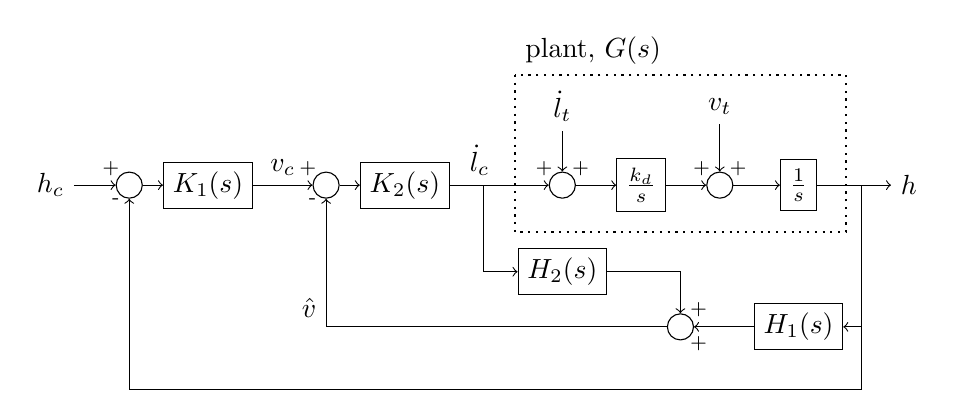
\begin{tikzpicture}[scale=2,
     block/.style = {draw, rectangle,node distance=1cm},
     input/.style = {node distance=1cm},
     output/.style = {node distance=1cm},
     arrow/.style={draw, -latex,node distance=2cm},
     pinstyle/.style = {pin edge={latex-, black,node distance=2cm}},
     sum/.style = {draw, circle, node distance=1cm},
     gain/.style = {regular polygon, regular polygon sides=3,draw, fill=white, text width=1em,
      inner sep=0mm, outer sep=0mm,
      shape border rotate=-90}
    ]
        
    \node [input] (hcmd) {$h_c$};
    \node [sum,right of=hcmd] (hsum) {};    
    \node [block,right of=hsum, node distance=1cm] (K1) {$K_1(s)$};
    \node [sum,right of=K1, node distance=1.5cm] (vsum) {};
    \node [block, right of=vsum] (K2) {$K_2(s)$};
    \node [sum, right of=K2, node distance=2cm] (dlift) {};
    \node [input, above of=dlift] (ldist) {$\dot l_t$};
    \node [block, right of=dlift] (lint) {$\frac{k_d}{s}$};
    \node [sum, right of=lint] (velocity) {};
    \node [input, above of=velocity] (vdist) {$v_t$};
    \node [block, right of=velocity] (vint) {$\frac{1}{s}$};
    \node [output, right of=vint,node distance=1.4cm] (h) {$h$};
    \node [block, below of=vint,node distance=1.8cm] (H1) {$H_1(s)$};
    \node [block, below of=dlift,node distance=1.1cm] (H2) {$H_2(s)$};
    \node [sum, left of=H1,node distance=1.5cm] (fsum) {};

    \draw[->] (hcmd) -- (hsum) node [above left] {\scriptsize +};
    \draw[->] (hsum) -- (K1);
    \draw[->] (K1) -- node [above] {$v_c$} (vsum) node [above left] {\scriptsize +};
    \draw[->] (vsum) -- (K2);
    \draw[->] (K2) -- node [above left] {$\dot l_c$} (dlift)  node [above left] {\scriptsize +};
    \draw[->] (ldist) -- (dlift) node [above right] {\scriptsize +};
    \draw[->] (dlift) -- (lint);
    \draw[->] (lint) -- (velocity) node [above left] {\scriptsize +};
    \draw[->] (vdist) -- (velocity) node [above right] {\scriptsize +};
    \draw[->] (velocity) -- (vint) node [above right] {};
    \draw[->] (vint) -- (h) node [above right] {};
    \draw  (h) ++ (-.3,0) -- ++(0,-1.3) coordinate (fb);
    \draw[->]  (h) ++ (-.3,0) |- (H1);
    \draw[->] (K2) ++ (0.5,0) |- (H2);
    \draw[->] (H1) -- (fsum) node [below right] {\scriptsize +};
    \draw[->] (H2) -| (fsum) node [above right] {\scriptsize +}; 
    \draw[->] (fsum) -| node [above left] {$\hat v$} (vsum) node [below left] {\scriptsize -};
    \draw[->] (fb) -| (hsum) node [below left] {\scriptsize -};
    \draw[thick,dotted] ($(dlift)+(-.3cm,.7cm)$) node [above right] {plant, $G(s)$} rectangle ($(vint)+(.3cm,-.3cm)$) ;

\end{tikzpicture}\\
\vspace{0.5cm}
\begin{tabular}{r l}
$K_1(s) = K_h$ & proportional altitude loop compensator \\
$K_2(s) = K_v$ & proportional velocity loop compensator \\ 
$H_1(s)$ & veloctiy estimator, lowpass filter on derivative of position\\
$H_2(s)$ & estimator of effect of changes in lift \vspace{.3cm}\\
$h_c$ & commanded altitude \footnotesize (set by Flight Controller) \\
$v_c$ & commanded velocity \footnotesize (output of position loop) \\
$\dot l_c$ & commanded change in lift per unit time  \footnotesize (output of velocity loop)\\
$\dot l_t$ & atmospheric disturbances that change balloon lift  \footnotesize (heating/cooling)\\
$v_t$ & atmospheric disturbances that change balloon velocity \footnotesize (turbulence)\\
$\hat v$ & estimate of velocity\\
$h$ & actual balloon altitude\\

\end{tabular}
\end{figure}

``Plant'' or $G(s)$ refers to the \emph{system} (atmosphere + balloon) dynamics, whereas everything else represents the control feedback structure that is computed in the ValBal flight code.


\newpage
\subsection{Constants Definitions for Code}
\begin{table}[h!]
\rmfamily
\begin{tabular}{l r  l} 
\sffamily \textbf{Contstant} &\sffamily \textbf{Default} &\sffamily \textbf{Description} \\

{\ttfamily freq}              & 20 & frequency that the controller is called at (Hz) \\
{\ttfamily k\_v            }  & 1e-3  & velocity Gain \\
{\ttfamily k\_h            }  & 1.5e-3  & altitude Gain   \\
{\ttfamily b\_dldt         }  & 6e-4  & lift rate of ballast actions (kg/s) \\
{\ttfamily v\_dldt         }  & 3e-3  & lift rate of valve actions  (kg/s) \\
{\ttfamily b\_tmin         }  & 5  & minimum ballast interval (s)   \\
{\ttfamily v\_tmin         }  & 5  & minimum valve interval (s)\\
{\ttfamily h\_cmd          }  & 13000  & commanded altitude (m)   \\
{\ttfamily kfuse           }  & 7  & atmosphere gain for velocity estimator   \\
{\ttfamily kfuse\_val      }  & 0.5  & velocity estimator gain modifier for valve  \\
{\ttfamily ss\_error\_thresh} & 750  & error tollerance for deadband (m) \\
\end{tabular}
\end{table}

\section{Trajectory Control}

\end{document}

